%\newpage
\section{Abstraction of Neural Network as Probabilistic Graphical Model}\label{chap:NNabstraction}


In this section, we construct a Bayesian network out of a trained neural network. In the end, the Bayesian network captures the distribution of neuron valuations in terms of latent features encoded in each neural network layers, as well as their causal relationships.

\subsection{Extraction of Hidden Features}\label{sec:featureextraction}

Assume that some feature extraction technique such as PCA and ICA has been used to analyse the neuron activation vector $\textbf{v}_i$ of layer $i$ that are induced by  a given \emph{training set} \(D_{train}\).
This produces a set of feature mappings $\Features{i}=\{\lambda_{i,j}\}_{j \in \{1,…,t_i\}}$ for $t_i$ features, such that each $(\lambda_{i,j}: \layerdom{i} \rightarrow \featcomp{i}{j})$ maps the vector space $\layerdom i$ 
of neuron valuation into the $j$-th component of the feature space $\featdom_{i,j}$.
%The latter space is the product \(\featdom i ≝ \prod_{j\in{1,…,s_i}}{\featcomp i j}\mbox.\)

Actually, \Features{i} is such that the neuron values $\textbf{v}_i$ for any input \(\textbf{x} \in D_{train}\), can be transformed into a \mbox{\(t_i\)-}dimensional vector
\begin{equation}
  \langle\lambda_{i,1}\textbf{v}_i,…,\lambda_{i,t_i}\textbf{v}_i\rangle \in \featdom i
\end{equation}
where $\lambda_{i,j}\textbf{v}_i$ represents the \mbox{\(j\)-}th component of the value obtained after mapping the instance $\textbf{x}$ into the feature space.
%We will refer to the projection \(λ_{i, j}∘\textbf{v}_i(x)\) as the \emph{latent feature valuation induced by $\textbf{x}$ on component \featcomp i j}.
%
%\begin{leaveout}
%  In the context of a layer $i$ where values output by all neurons result from the application of a Rectified Linear Unit (ReLU), we will further identify the projection of the \emph{activation threshold} into the feature space as \(λ_{i}(0) ≝ 〈λ_{i,1}(0), …, λ_{i,t_i}(0)〉\mbox.\)
%\end{leaveout}
%
\begin{figure}[t!]
    \centering
    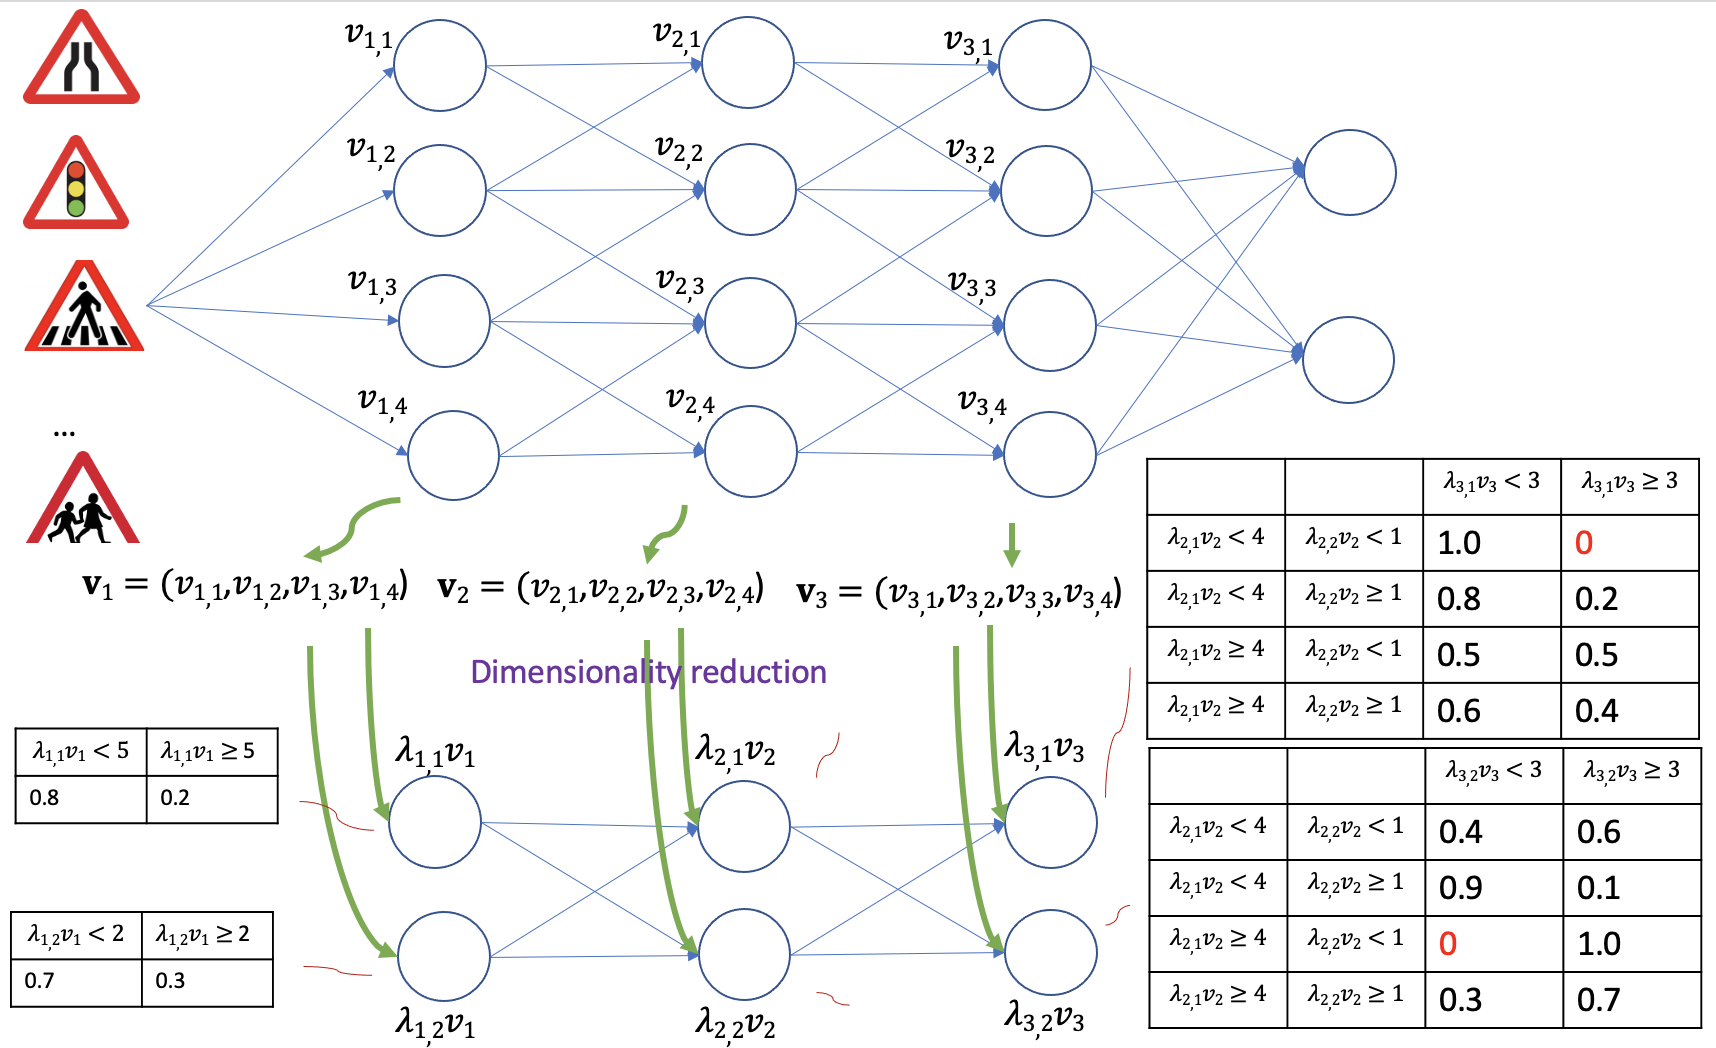
\includegraphics[width=\textwidth]{images/graphical models/diagram.png}
    \caption{Reducing Neural Networks to Bayesian Networks}
    \label{fig:diagram}
\end{figure}
%
Figure~\ref{fig:diagram} gives an illustrative diagram of reducing $\textbf{v}_1, \textbf{v}_2,\textbf{v}_3$ to features.
In particular, each $\textbf{v}_i$ is reduced to two features $\lambda_{i,1}\textbf{v}_i$ and $\lambda_{i,2}\textbf{v}_i$.


\subsection{Discretisation of Hidden Feature Space}\label{sec:discretisation}

The feature extraction techniques 
%mentioned in Section~\ref{sec:dimens-reduct-via} 
result in mappings $\lambda_{i,j}% \textbf{v}_i
$ that range over a continuous and potentially infinite domain.
%, such as ℝ.
Yet, Bayesian network-based abstraction technique relies on the construction of \emph{probability tables}, where each entry associates a set of \emph{distinct} latent feature values with a probability.
For this construction to be relevant, we therefore \emph{discretise} each latent feature component into a \emph{finite} set of sub-spaces.

%

\subsection{Construction of Bayesian Network Abstraction}
\label{sec:constr-bayes-netw}


The abstraction that we construct primarily represents the \emph{probabilistic distribution} of the set of latent feature values induced by a set $\textbf{X}$ of test instances.
In other words, given an input \(\textbf{x} \in 
\textbf{X}\), the abstraction allows us to estimate the probability that $\textbf{x}$ induces a given combination of values for the latent features that have been learned by the neural network.

Thanks to the layered and a\-cyclic nature of the neural networks that we consider, we can directly characterise the \emph{causal relationship} between the sets of neuron values in various layers \wrt a series of inputs as well.
In other words, given an input \(\textbf{x} \in 
\textbf{X}\), one can in principle estimate the conditional probability of each neuron value at layer $i$ \wrt the probability of every combination of neuron values at layer $i-1$.
By lifting the above relationship from individual neuron values to latent feature intervals, we seek to capture \emph{causal semantic relations} that link the features at each layer: in a layer $i$, and with an input $\textbf{x}$, the \emph{probability} that a latent feature valuation belongs to a given interval in the corresponding feature space is \emph{dependent} on probabilities pertained to latent feature intervals at layer $i-1$.



\subsection{Preserved Property}

First of all, we show that the constructed Bayesian network is an abstraction of the neural network.
Given a finite set $\textbf{X}$ of inputs, an abstraction constructs a set $\textbf{X}' \supseteq \textbf{X}$ that generalises $\textbf{X}$ to more elements \cite{DBLP:journals/corr/abs-1911-09032}. Given an input $\textbf{x}$ and a Bayesian network $\lambda(\textbf{X})$, we are able to check the probability of $\textbf{x}$ on $\lambda(\textbf{X})$, i.e., $\lambda(\textbf{X})(\textbf{x})$. We say that $\textbf{x}$ is included in $\lambda(\textbf{X})$ if $\lambda(\textbf{X})(\textbf{x})>0$.
The following lemma suggests that every sample in $\textbf{X}$ is included in $\lambda(\textbf{X})$:

\begin{lemma}\label{lemma:abstraction}
  All inputs $\textbf{x}$ in the dataset $\textbf{X}$ are included in the $\lambda(\textbf{X})$ with probability greater than 0.
\end{lemma}

Let $\textbf{X}'$ be the set of inputs that satisfy $\lambda(\textbf{X})(\textbf{x})>0$. This lemma suggests that $\textbf{X}'\supset \textbf{X}$. Therefore, $\lambda(\textbf{X})$ defines an abstraction of the dataset $\textbf{X}$.
This abstraction also suggests that the abstraction assumption -- \ie inputs that are outliers \wrt the abstraction are also outliers \wrt the original neural network -- is reasonable because $\textbf{X}'\supset \textbf{X}$.

In addition to this simple property, \cite{berthier2021abstraction,Alshareef2022} also consider other analysis techniques based on the abstracted Bayesian network. 

